%%%%%%%%%%%%%%%%%%%%%%%%%%%%%%%%%%%%%%%%%
% Beamer Presentation
% LaTeX Template
% Version 1.0 (10/11/12)
%
% This template has been downloaded from:
% http://www.LaTeXTemplates.com
%
% License:
% CC BY-NC-SA 3.0 (http://creativecommons.org/licenses/by-nc-sa/3.0/)
%
%%%%%%%%%%%%%%%%%%%%%%%%%%%%%%%%%%%%%%%%%

%----------------------------------------------------------------------------------------
%	PACKAGES AND THEMES
%----------------------------------------------------------------------------------------

\documentclass{beamer}

\mode<presentation> {

% The Beamer class comes with a number of default slide themes
% which change the colors and layouts of slides. Below this is a list
% of all the themes, uncomment each in turn to see what they look like.

%\usetheme{default}
%\usetheme{AnnArbor}
%\usetheme{Antibes}
%\usetheme{Bergen}
%\usetheme{Berkeley}
%\usetheme{Berlin}
%\usetheme{Boadilla}
%\usetheme{CambridgeUS}
%\usetheme{Copenhagen}
%\usetheme{Darmstadt}
\usetheme{Dresden}
%\usetheme{Frankfurt}
%\usetheme{Goettingen}
%\usetheme{Hannover}
%\usetheme{Ilmenau}
%\usetheme{JuanLesPins}
%\usetheme{Luebeck}
\usetheme{Madrid}
%\usetheme{Malmoe}
%\usetheme{Marburg}
%\usetheme{Montpellier}
%\usetheme{PaloAlto}
%\usetheme{Pittsburgh}
%\usetheme{Rochester}
%\usetheme{Singapore}
%\usetheme{Szeged}
%\usetheme{Warsaw}

% As well as themes, the Beamer class has a number of color themes
% for any slide theme. Uncomment each of these in turn to see how it
% changes the colors of your current slide theme.

%\usecolortheme{albatross}
%\usecolortheme{beaver}
%\usecolortheme{beetle}
%\usecolortheme{crane}
%\usecolortheme{dolphin}
%\usecolortheme{dove}
%\usecolortheme{fly}
%\usecolortheme{lily}
%\usecolortheme{orchid}
%\usecolortheme{rose}
%\usecolortheme{seagull}
%\usecolortheme{seahorse}
%\usecolortheme{whale}
%\usecolortheme{wolverine}

%\setbeamertemplate{footline} % To remove the footer line in all slides uncomment this line
%\setbeamertemplate{footline}[page number] % To replace the footer line in all slides with a simple slide count uncomment this line

%\setbeamertemplate{navigation symbols}{} % To remove the navigation symbols from the bottom of all slides uncomment this line
}

\usepackage{graphicx} % Allows including images
\usepackage{booktabs} % Allows the use of \toprule, \midrule and \bottomrule in tables

%----------------------------------------------------------------------------------------
%	TITLE PAGE
%----------------------------------------------------------------------------------------

\title[DBMS]{My experience in data management systems and public engagement activities} % The short title appears at the bottom of every slide, the full title is only on the title page

\author{Saumya Bhatnagar} % Your name
%\institute[Data Engineering] % Your institution as it will appear on the bottom of every slide, may be shorthand to save space
%{
%University of California \\ % Your institution for the title page
%\medskip
%\textit{john@smith.com} % Your email address
%}
\date{\today} % Date, can be changed to a custom date

\begin{document}

\begin{frame}
\titlepage % Print the title page as the first slide
\end{frame}


%----------------------------------------------------------------------------------------
%	PRESENTATION SLIDES
%----------------------------------------------------------------------------------------

%------------------------------------------------
\section{DBMS} % Sections can be created in order to organize your presentation into discrete blocks, all sections and subsections are automatically printed in the table of contents as an overview of the talk
%------------------------------------------------


\subsection{MySql, Oracle, Cassandra, HBase, MongoDB} % A subsection can be created just before a set of slides with a common theme to further break down your presentation into chunks

\begin{frame}
	\frametitle{Why DBMS!}
		\begin{block}{Users}
		\begin{table}
			\begin{tabular}{l l l}
				%\toprule
				\textbf{DBA} & \textbf{APP PROGRAMMERS} & \textbf{END USERS}\\
				\midrule
				DB Schema & App Software & Query App Interface \\
				%\bottomrule
			\end{tabular}
		\end{table}
		\end{block}
	
	\begin{block}{DBMS}
	\begin{table}
		\begin{tabular}{l l l}
			%\toprule
			\textbf{Query Processor} & Query Evaluation Engine (DDL Interpreter,\\ 
			 & DML Compiler, Application Object Code) \\
			\midrule
			\textbf{Storage Manager} & Buffer Manager, File Manager, \\ & Transaction Manager \\
			%\bottomrule
		\end{tabular}
	\end{table}
	\end{block}

	\begin{block}{Database}
	Data files, Data Dictionaries, Indices
	\end{block}

\end{frame}

%------------------------------------------------

\begin{frame}
\frametitle{DBMS Types}
	\begin{table}
		\begin{tabular}{l | c | c }
			  & SQL & NoSQL \\
			\hline 
			High Level Model & ER Model &  \\ 
			\hline
			Representational Model & Hierarchical (IMS), \\  & Relational (Oracle, DB2, SQL Server), \\  & Network (IDMS, IMAGE) &  \\
			\hline
			Low-Level Model &   & \\
			
		\end{tabular}
		%\caption{Triathlon results}
	\end{table}


	DB Architectures
	\begin{itemize}
		\item Centralized DBMS Architecture
		\item Client-Server Architecture
		\item Distributed Database Architecture
	\end{itemize}

	Schema Types
	\begin{itemize}
		\item Internal Schema
		\item Conceptual Schema
		\item External Schema
	\end{itemize}

\end{frame}

%------------------------------------------------

\begin{frame}
\frametitle{Glossary on Keys}
	Key Types
	\begin{itemize}
		\item Super Key
		\item Candidate Key
		\item Primary Key
		\item Secondary Key
		\item Foreign Key
		\item Composite Key
		\item Compound Key (Composite key with foreign key)
		\item Alternate Key
		\item Sort/Control Key
		\item Surrogate key
	\end{itemize}
\end{frame}


%------------------------------------------------

\begin{frame}
\frametitle{Overview} % Table of contents slide, comment this block out to remove it
\tableofcontents % Throughout your presentation, if you choose to use \section{} and \subsection{} commands, these will automatically be printed on this slide as an overview of your presentation
\end{frame}



%------------------------------------------------


\section{Hadoop}
\subsection{Hadoop Ecosystem}
\subsection{External Data Storages}
\subsection{Query Engines}


\begin{frame}
\frametitle{Hadoop Ecosystem}
\begin{figure}
	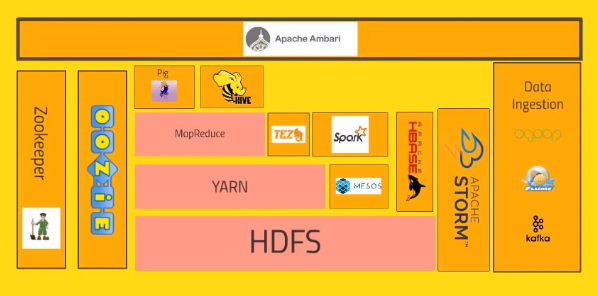
\includegraphics[scale=0.8]{hadoop}
	%\caption{Hadoop Ecosystem}
\end{figure}

\end{frame}

\begin{frame}
\frametitle{Query Engines And External data storage}
\begin{figure}
	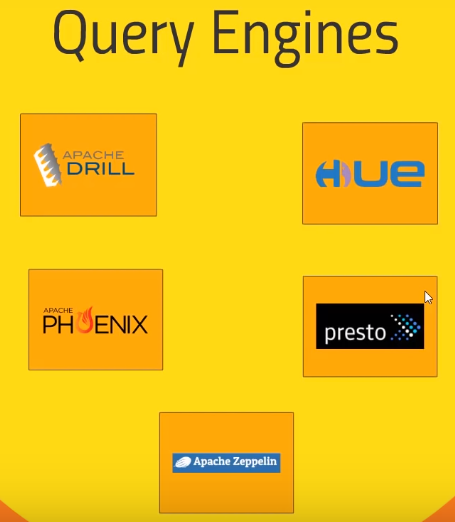
\includegraphics[scale=0.45]{QueryEngines}
	%\caption{Query Engines}
	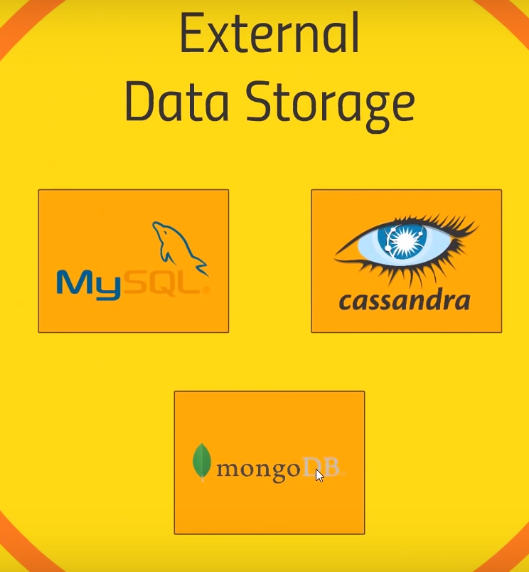
\includegraphics[scale=0.45]{ExternalDataStorage}
	%\caption{Hadoop Ecosystem}
\end{figure}
\end{frame}


\begin{frame}
\frametitle{Clustered Computing Platforms (Mapreduce, Spark)}
	SPARK
	\begin{itemize}
		\item Distributing queries and trend analysis
		\item Microbatching for historical analysis
		\item Loading large datasets into memory
		\item Running queries against large datasets
	\end{itemize}
\end{frame}


\section{Which Data Storage?}

\begin{frame}
\frametitle{Pros \& Cons of the databases}
	\begin{table}
		\begin{tabular}{l | c }
			\hline
			Hadoop/Mapreduce & Slow for real time analytics \\
			\hline 
			MongoDB & Global write lock performance concerns \\ 
			\hline 
			Cassandra (w/o solr) & Query Limitations \\
			\hline 
			Cassandra (w/o solr) & No bother about denormalizing, \\  & duplication, access pattern data modelling \\
			\hline 
			Solr & Search capabilities, partial text search, \\  & facet queries, geospatial, etc.\\
			\hline
		\end{tabular}
		%\caption{Pros \& Cons of the databases}
	\end{table}
\end{frame}



\begin{frame}
\frametitle{Which Data Storage?}
\begin{figure}
	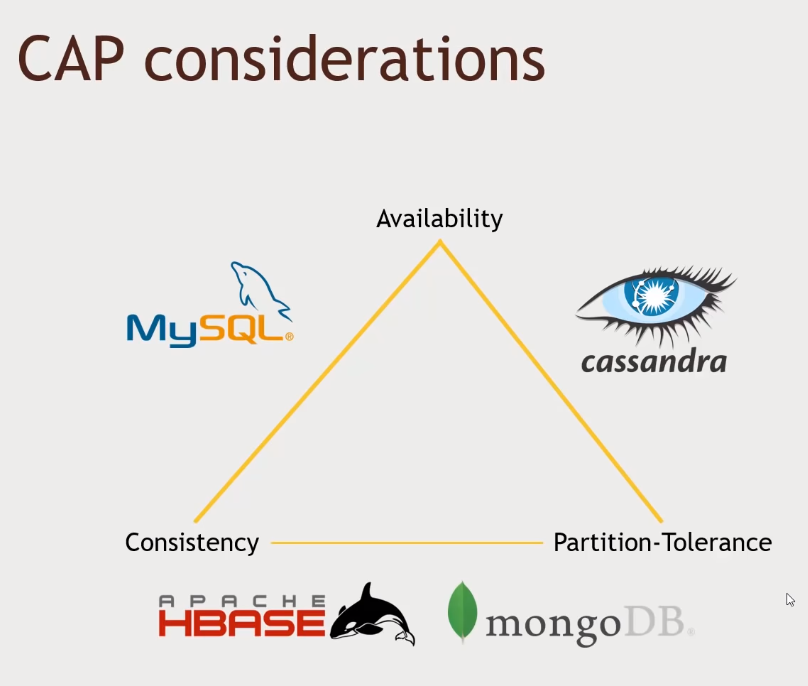
\includegraphics[scale=0.4]{CAP}
	%\caption{Hadoop Ecosystem}
\end{figure}
\end{frame}


\section{SQL}
\subsection{MySql, Vertica}



%------------------------------------------------

%------------------------------------------------
\begin{frame}[fragile] % Need to use the fragile option when verbatim is used in the slide
\frametitle{Vertica for Big Data Engineering}

\begin{columns}[c] % The "c" option specifies centered vertical alignment while the "t" option is used for top vertical alignment
	
	\column{.3\textwidth} % Left column and width
	\textbf{Command Type}
	\begin{enumerate}
		\item DDL
		\item DML
		\item DCL
		\item TCL
	\end{enumerate}
	
	\column{.6\textwidth} % Right column and width
	\begin{enumerate}
		\item create, alter, drop, truncate, rename
		\item select, insert, update, delete
		\item grant, revoke
		\item commit, rollback
	\end{enumerate}
	
\end{columns}


\begin{example}[Vertica Code Example]
	\begin{verbatim}
	SELECT name, class, date, 
	RANK() OVER (PARTITION BY class ORDER BY marks desc) AS rank 
	FROM student 
	WHERE name IS NOT NULL 
	AND subject like 'math%' 
	AND date > '01/01/2007' 
	ORDER BY class;
	\end{verbatim}
\end{example}


\end{frame}


%------------------------------------------------
\begin{frame}
\frametitle{SQL Glossary}
\begin{itemize}
	\item bandwidth=rate of data transfer
	\item latency=time of date transfer
	\item 1NF, NF, 3NF, BCNF
	\item ACID Properties (atomicity, consistency, isolation, durability)
	\item Lossless Decomposition
	\item Data Independence
	\item 
	\item 
	\item 
	\item 
	\item 
	\item 
\end{itemize}
\end{frame}

%------------------------------------------------

\section{NoSQL}
\subsection{Cassandra with solr}
\subsection{No one single point of failure}

%------------------------------------------------

\begin{frame}
\frametitle{DSE provides integration between Cassandra with Solr}
	\begin{itemize}
		\item Storage grid (cassandra) + Search grid(solr)
		\item Devcenter or cqlsh
		\item Cassandra cluster handling over 1TB data
		\item 2 Data Centers
		\item 3 Servers, with RF of 3
		\item configure dse.yaml or vassandra.yaml
		\item Opscenter
		\item Solr Admin UI gives Solr Index Size
		\item All Nodes should have solr enabled within DC
		\item Map collection to dynamic fields
		\item solr queries have consistency levels
	\end{itemize}

\end{frame}

\begin{frame}[fragile]
\frametitle{CQL syntax similar to SQL syntax}
	\begin{example}[CQL Code Example]
		\begin{verbatim}
		/*create table defining partition, clustering keys*/
		CREATE TABLE student ( 
		name text, class text, subject text, date timestamp,
		PRIMARY KEY ((name, class), date) 
		);
		\end{verbatim}
	\end{example}
	Primary key is defined as ((partition keys), clustering/sorting keys)
	\begin{example}[CQL Code Example]
		\begin{verbatim}
		SELECT name, class, date, rank FROM student 	
		WHERE name IS NOT NULL 
		AND subject CONTAINS 'math' 
		AND date > '01/01/2007' 
		ORDER BY class
		PER PARTITION LIMIT 2;
		\end{verbatim}
	\end{example}
\end{frame}

%------------------------------------------------

\begin{frame}[fragile]
\frametitle{Solr provides full text search, term-search}
\begin{example}[CQL + Solr Code Example]
	\begin{verbatim}	
	SELECT name, class, date
	FROM student WHERE 
	solr_query='{"q":"name:[* TO *] AND subject:math*",
	             "fq":"date:[2007-01-01T00:00:00Z TO NOW]",
	             "facet":{"field":"class"},
	             "sort":"class, marks desc", 
	             "paging":"driver", 
	             "timeAllowed":30000 }'
	ALLOW FILTERING;
	\end{verbatim}

\end{example}

Clustering columns can be defined in WHERE clauses if ALLOW FILTERING is also used even if a secondary index is not created

\end{frame}


\begin{frame}
\frametitle{Cassandra Glossary}
\begin{itemize}
	\item snitch
	\item Gossip
	\item Quorum
	\item num\_tokens
	\item max\_solr\_concurrency\_per\_core = cpu code / num solr cores
	\item partitioner
	\item auto\_bootstrap  
	\item 
	\item 
	\item 
	\item 
	\item 
\end{itemize}
\end{frame}





%------------------------------------------------

\section{APIs}
\begin{frame}\frametitle{SOAP vs REST}
	Client (Machine Devices - Mobile, desktop) $\rightarrow$ API Binding $\rightarrow$ Server\\

	SOAP:\\
	\begin{itemize}
		\item Stateless
		\item Slow
		\item XML
	\end{itemize}
	REST:\\
	\begin{itemize}
		\item Public
		\item Fast
		\item Multiple formats
	\end{itemize}
\textbf{REST}:\\
NODE.js\\
MongoDB (native js code) - JS based\\
json format\\
MongoDB: 2 collection joins, aggregation in mongoDB\\instead js for loop can be used\\


\end{frame}

\begin{frame}\frametitle{REST vs Bulk}
	Bulk is built on top of REST\\
	Bulk:\\
	\begin{itemize}
		\item async
		\item batches
	\end{itemize}	
\end{frame}

\begin{frame}\frametitle{Email API}
	Email uses SMTP and Port number\\
	Tight coupling\\
	IOC (Inversion of Control):\\
	Inject email in customer:
	1. Property in class
	2. Parameter
\end{frame}

\begin{frame}\frametitle{CQRS}
	command\\
	...\\
	read\\
	...
\end{frame}

\begin{frame}\frametitle{API gateway}
	Swagger\\
	APIGEE:\\
	\begin{itemize}
		\item authentication control
		\item traffic control
	\end{itemize}
	Server info... API gateway provides URL
\end{frame}



%------------------------------------------------


%------------------------------------------------

\section{Microservices}

\begin{frame}
	\frametitle{Microservices}
	Microservices architecture runs on top of STORM/JMS/KAFKA \newline
	Storm (handles clustering/distribution) \newline
	Kafka (messaging between the grids) \newline
	Kafka or Rabbit NQ are message broker URIs\\
	for cache use Redis. Redis is a cache DB\\
	JWT (Json Web token): network calls to DB should be least $\rightarrow$ Resource Management\\
	YAML $\rightarrow$ dependent on other services. has details such as name, port, URL, env variables, etc.
\end{frame}


\begin{frame}\frametitle{Docker - Container}
	Docker is OS\\
	Containers are VM ware\\
	Cluster has nodes. Nodes has pods. e.g. Pod1, Pod2, Pod3, Pod4 are 4 containers. Pod1 may act as Inst of Service\\
	Dockerfile is image of service and is "Built, deployed and ran" by DevOps\\
\end{frame}

\begin{frame}\frametitle{Domain Driven Design}
	Service bus\\
	Rabbit MQ\\
	%\vspace{10}
	Order Service \& Domain Service

	DDD: Command (message) $\rightarrow$ Event [Eventual Consistency]\\
	
	Service bus... message sent to exchange queue via routing key
\end{frame}

\begin{frame}\frametitle{Pub/Sub Design Pattern}
content...
\end{frame}


\begin{frame}\frametitle{title}
content...
\end{frame}

\begin{frame}\frametitle{Microservices on Docker}
	content...
\end{frame}

\begin{frame}\frametitle{Microservices on Kubernetes}
content...
\end{frame}

\begin{frame}\frametitle{Serverless}
content...
\end{frame}




\begin{frame}
\Huge{\centerline{Thank You!}}
\end{frame}

%----------------------------------------------------------------------------------------

\end{document} 